\documentclass{article} % For LaTeX2e
\usepackage{nips15submit_e,times}
\usepackage{hyperref}
\usepackage{url}
%\documentstyle[nips14submit_09,times,art10]{article} % For LaTeX 2.09

\usepackage{graphicx}
\title{Weekly Report(July.1.2019-July.7.2019)}


% The \author macro works with any number of authors. There are two commands
% used to separate the names and addresses of multiple authors: \And and \AND.
%
% Using \And between authors leaves it to \LaTeX{} to determine where to break
% the lines. Using \AND forces a linebreak at that point. So, if \LaTeX{}
% puts 3 of 4 authors names on the first line, and the last on the second
% line, try using \AND instead of \And before the third author name.

\newcommand{\fix}{\marginpar{FIX}}
\newcommand{\new}{\marginpar{NEW}}

%\nipsfinalcopy % Uncomment for camera-ready version

\begin{document}


\maketitle

\begin{abstract}
This week I spend some time to build my environment on Linux and build a very simple demo for AlexNet.
\end{abstract}

\section{Work Environment}
Since the main memory of my computer is only 4G, it's really slow to run code on Linux, which is installed on HDD. So I used to run code in Windows. However, it's troublesome to configure some environment variables. So i decide to run code on Linux now. This week I just spend some time to install all the corresponding softwares and configur correctly. I also try to build a sample network from Alex Net. Although it wworks with many bugs.

\subsection{NVIDIA} 
use order "lspci | grep -i nvidia" to see the GPU version.

\subsection{Anaconda3} 
Download the Anaconda3 installation package which python version is 3.7 on the following website. Install it as requested.

\begin{center}
	\url{https://www.anaconda.com}
\end{center}

Since I did some modification on my terminal, I use zsh instead of bash, therefore I encountered a problem "zsh: command not found: conda". To solve it, I add "export PATH="/home/rsp/anaconda3/bin:\$PATH" in the file loacted in the file path "~/.zshrc", then type "source ~/.zshrc" to activate it.

\subsection{virtualenv}
Since we have installes Anaconda3, we can create an independent environment by the order "conda create -n env-name python=3.6", type "conda activate env-name" to get into the virtual environment, and focus on our work after installing some compulsory python libraries.

"conda deactivate" can get out of the virtual environment, and "conda remove -n env-name" can remove the virtual environment at all.

\subsection{Pytorch}
I encountered a big problem here, which cost me for a night and I still can't solve it. Finally I consult to my roomate Ni, he solved it for me. I really appreciate it.

The problem is I can't use gpu after installing cuda and cuDnn. At first I install latest version, it didn't works. So I removed them and installed version 9.0 instead, but it still didn't work. I checked for several times but  can't know why. Finally it's caused by the pytorch, which I installed long time ago, I even forgot it. Reinstall pytorch with a lower version, it works!

\section{paragraph}
I think image classification is a process that for a given dataset, we use classification methods to try to divide them into different parts. Accuracy is to measure a method is good or not. We want to get a classification result with a good accuracy, so we need to keep trying to find a optimal method.

About my plan, actually I didn't have a very concrete plan. In general, I will obey the requirements given in miniproject and finish them step by step. First is the AlexNet, I plan to use one more week working on it. Then the pre-trained model, I plan to working on it until the end of summer semester.

\section{AlexNet Demo}

\begin{figure}[ht]
	\centering  %插入的图片居中表示
	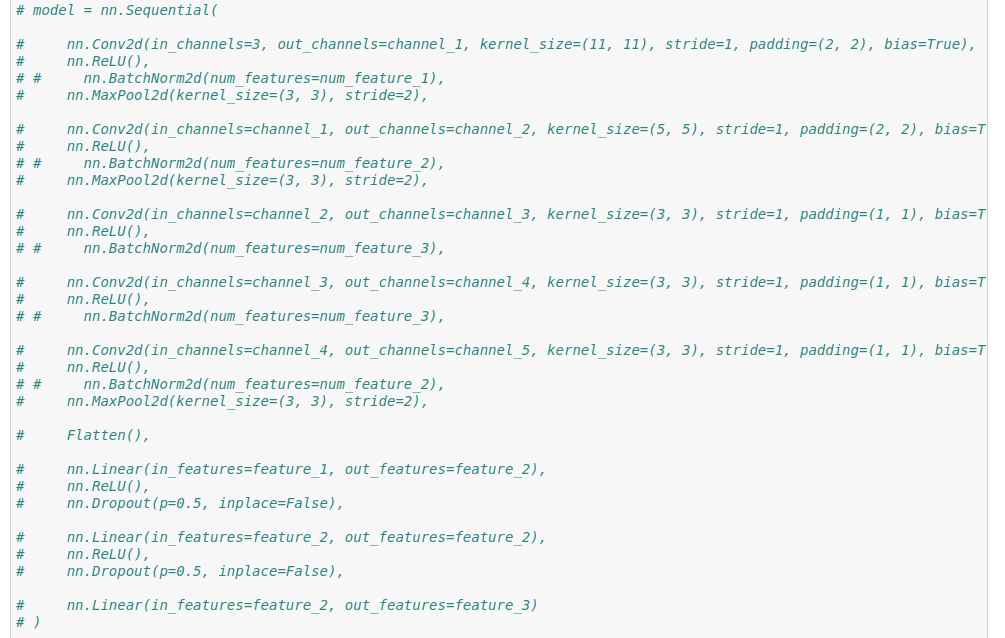
\includegraphics[width=1\textwidth]{1.png} 
	\caption{AlexNet}  %图片的名称
	\label{fig:f1}   %标签,用作引用
\end{figure}

\begin{figure}[ht]
	\centering
	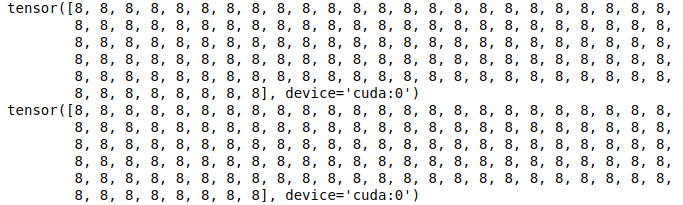
\includegraphics[width=1\textwidth]{2.png}
	\caption{prediction output}
	\label{fig:f2}
\end{figure}


I build a classic AlexNet like this, but a question puzzles me. The size of the images for training are all 3*32*32, but in the classic AlexNet, the size of input image are 3*227*227. I can't figure out why they are different. And if it's the truth, how should I appply this dataset to train classic AlexNet? I know "torchvision.transforms" can resize the image, but I searched for this and didn't find someone else did such operation when training AlexNet. So does it necessary to resize it or use some other methds?

Another problem is I can't get a reasonable accuracy. I build the net and train it use the code above, but the outputs are always similar. Since the input is too big, I will show you the predict labels. They are always the same number, which varies from 0 to 9, corresponding to the number of classes. I thought the resize operation may cause this result, so I comment it and rebuild the net. The results are still the same. I think it may be caused by trainning process code, but I can't figure out why.

\begin{figure}[ht]
	\centering
	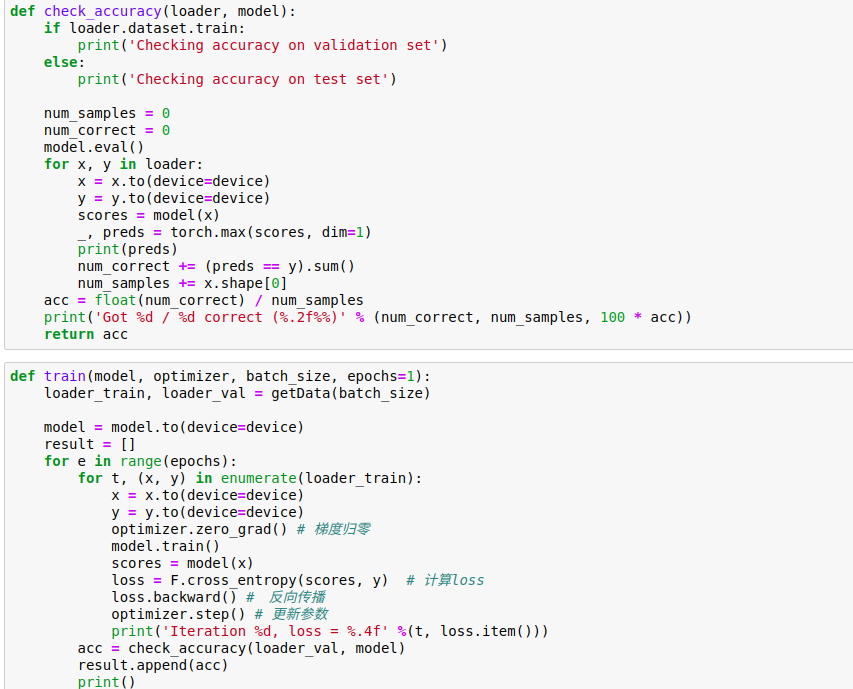
\includegraphics[width=1\textwidth]{3.png}
	\caption{main training process}
	\label{fig:f3}
\end{figure}

\section{Plan}
I will appreciate it so much if someone can answer these questions for me so that I can start to solve next porblem. The sooner, the better.

\end{document}
